\documentclass[12pt,oneside]{article}
\usepackage{enumerate}
\usepackage{fancyhdr}
\usepackage{a4wide}
\usepackage{titlesec}
\usepackage{enumitem}
\usepackage[utf8]{inputenc}
\usepackage{graphicx} % Required for inserting images
\usepackage{tocloft}
\usepackage[table]{xcolor}
\usepackage{ragged2e}

\setlength{\arrayrulewidth}{0.5mm}
\setlength{\tabcolsep}{10pt}
\renewcommand{\arraystretch}{2.5}

\usepackage{longtable}
\definecolor{lightblue}{HTML}{b0c4de}
\definecolor{lightsteelblue}{HTML}{add8e6}

\usepackage{hyperref}

\usepackage{floatrow} 
\usepackage{graphicx}
\usepackage[export]{adjustbox}
\usepackage{wrapfig}

%%%%%%%%%%%%%%%%%%%%%%%%%%%%%%%%
\begin{document}

%pagina introduttiva
\begin{titlepage}
    \begin{flushright}
        \textbf{Corso di Fondamenti di Intelligenza Artificiale}
        \textbf{\\Università degli Studi di Salerno}
    \end{flushright}
    \vspace*{1.5cm}
    \centering
    \includegraphics[width=0.4\textwidth]{logoUNISA.png}
    \vfill
    \Huge\textbf{BOOKS}
    \vspace{1ex}
    \rule{\linewidth}{1pt}
    \Large\textbf{Maria Angela Mancuso \\
        Ines Malfettone \\
        Federico Santonicola \\
        Attilio Sessa}
    \vfill
    \today
\end{titlepage}

%indice
\clearpage %crea nuova pagina

\setcounter{page}{1}

\begin{flushright}
        \Large\textbf{Indice}
\end{flushright}
\rule{\linewidth}{1pt}

\renewcommand{\contentsname}{}
\tableofcontents

%1
\clearpage
\setcounter{section}{0}
\section{Introduzione}
    \begin{enumerate}
    \subsection{Scopo del progetto}
    \begin{justify}
    
        Il nostro progetto si pone come obiettivo lo studio e la sperimentazione di differenti tecniche di Machine Learning capaci di analizzare ed estrarre informazioni da dati sotto forma di linguaggio naturale. Nello specifico si è interessati alla categorizzazione di libri tramite una breve descrizione testuale ed un elenco di autori. La categorizzazione è stata elaborata tramite due tecniche di Machine Learning, Classificazione e Clustering, che, seppur facenti utilizzo di due approcci diversi (rispettivamente apprendimento supervisionato e apprendimento non supervisionato), in linea teorica dovrebbero essere in grado di riportare risultati similari e confrontabili. A tal proposito occorrerà addestrare più modelli differenti per entrambe le tecniche e verificare quali di questi permette di ottenere il miglior risultato.

    \end{justify}
    \end{enumerate}

\section{Specifiche del progetto}
    \begin{enumerate}
        \subsection{Ambiente: PEAS}
    \begin{flushleft}
        Specifica PEAS
    \end{flushleft}
   
%tabella
    \centering
    \begin{longtable}{ | p{3cm} | p{11cm} | }\hline
    \multicolumn{2}{|c|}{PEAS} \\ \hline
    \rowcolor{lightblue}
    Performance & La misura di prestazione è la capacità di avvicinarsi quanto più possibile al corretto genere del libro in questione. È necessario utilizzare misure di prestazione differenti per valutare Classificazione e Clustering. Nel caso della Classificazione si è usato: Accuratezza, Report di classificazione, che comprendono Precisione, Recall e F1-score per ciascuna classe, e una Matrice di  confusione. Per il clustering, invece,  si è utilizzato il Silhouette Score.\\
    \hline
    \rowcolor{lightsteelblue}
    \textbf{Environment} & I nostri modelli sono stati realizzati e operano nell'ambiente di sviluppo PyCharm il quale presenta le seguenti caratteristiche: \begin{itemize}
        \item \textbf{completamente osservabile}: il modello ha la visione completa del dataset e degli attributi associati a ciascun libro.
        \item \textbf{deterministico}: una volta addestrato un modello, la variazione dello stato dell'ambiente rimane la stessa a fronte degli stessi input.
        \item \textbf{episodico}: l'agente delibera a fronte di determinati episodi che consistono in nuove richieste di predizione.
        \item \textbf{statico}: l'ambiente resta invariato mentre l'agente opera.
        \item \textbf{discreto}: viene fornito un insieme discreto di informazioni per ciascun libro.
        \item \textbf{singolo}: l'ambiente permette di addestrare più modelli ma questi vengono valutati singolarmente.
    \end{itemize}
    \hline
    \rowcolor{lightblue}
    \textbf{Actuators} & Gli agenti mostrano i risultati attraverso due tipi di attuatori: \begin{itemize}
    \item console dell'ambiente di sviluppo: durante l'addestramento e testing i modelli riportano informazioni di controllo e i risultati ottenuti.
    \item grafici esplicativi: mostrano informazioni di vario tipo, tra cui analisi del dataset e risultati ottenuti dalle predizioni dei modelli.\end{itemize}
    \hline
    \rowcolor{lightsteelblue}
    \textbf{Sensors} & I modelli ricevono le informazioni necessarie per l'addestramento tramite un file contenente il dataset. Inoltre è possibile specificare tramite console nuovi dati su cui effetturare nuove predizioni. \\
    \hline
    
    \end{longtable}
   \caption{Tabella della specifica PEAS}
\label{table:ta}
\end{enumerate}

    

\section{Analisi e preparazione dei dati}
    \begin{enumerate}
    \subsection{Scelta del dataset}
    \begin{justify}
    Per lo scopo di tale progetto si è scelto un dataset già esistente, reperibile \href{https://www.kaggle.com/datasets/elvinrustam/books-dataset}{qui}. La ricerca del dataset si è basata sulla necessità di trovarne uno contenente libri provveduti di descrizione e autori. Il dataset fornisce informazioni relative a 103063 libri ed ha una dimensione di 69.75MB. Tutti i dati sono in formato testuale. Inizialmente presentava 7 features diverse (Title, Authors, Description, Category, Publisher, Publish Date, Price) ma per lo scopo del nostro progetto abbiamo ritenuto sufficiente considerare solo le seguenti features: Title, Authors, Description, Category.  
    \end{justify}
    \end{enumerate}

    \begin{enumerate}
    \subsection{Data cleaning}
    \begin{justify}
    Il Data Cleaning è la fase durante la quale ci si occupa di "pulire" il dataset mantenendo solo i dati più completi e chiari. Da una prima analisi del dataset si è rilevata la presenza di campi nulli per alcune righe e la presenza della stessa descrizione di default (inserita dall'autore del dataset) ripetuta in una parte dei libri. La presenza di questa descrizione di default può ostacolare l'esecuzione delle tecniche di classificazione e degli algoritmi di clustering che saranno implementate successivamente. Per ovviare a questi problemi è stata eseguita un'eliminazione delle righe con campi nulli e delle righe duplicate. Tutte queste operazioni sono state svolte tramite la funzione "cleanData". Come risultato si è ottenuto un dataset composto da sole descrizioni significative.
    \end{justify}
    \includegraphics[width=0.95\textwidth]{cleanData.png}
    \end{enumerate}

    \begin{enumerate}
    \subsection{Bilanciamento dataset}
    \begin{justify}
    Da una prima osservazione del grafico, che mostra i libri divisi nei 20 generi, si può notare che il dataset è sbilanciato. Quindi, per ovviare a problemi di overfitting, si è ritenuto necessario bilanciare il dataset quanto più possibile. Ciò è stato fatto tramite l'utilizzo della funzione "balanceCategories", la quale verifica il numero di righe per ogni categoria ed elimina casualmente delle righe di categorie con più di 'threshold' esempi.
    \end{justify}
    \includegraphics[width=0.95\textwidth]{balanceCategories.png}
    \begin{justify}
    Si passa da un dataset aventi i seguenti dati iniziali:
    \end{justify}
    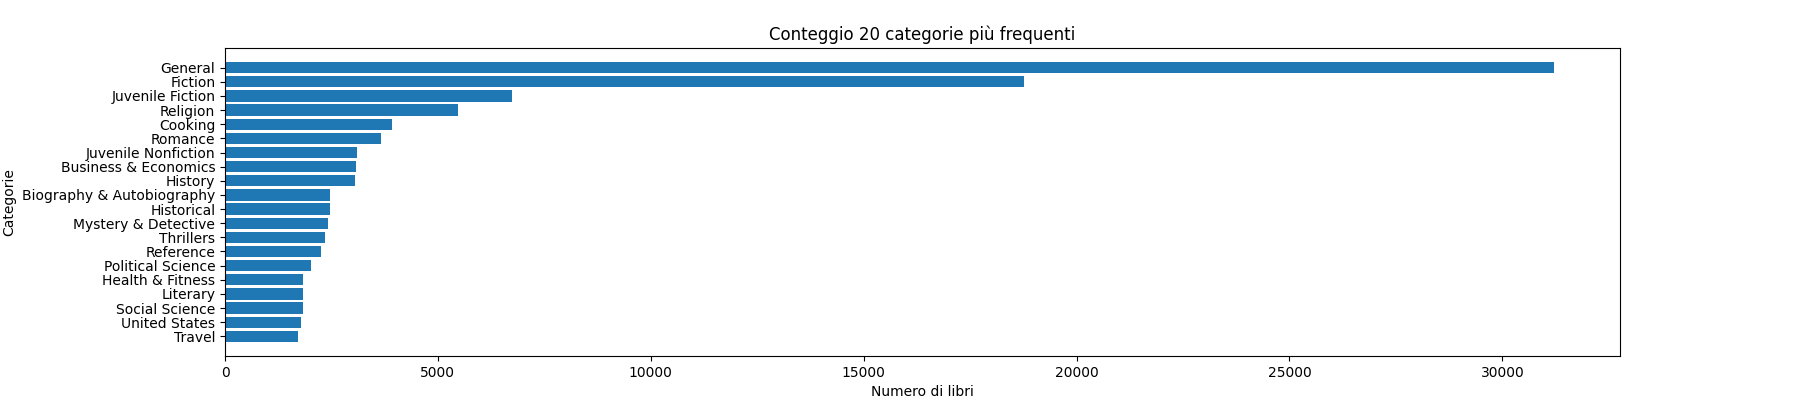
\includegraphics[width=0.96\textwidth]{dati_iniziali.png}
    \begin{justify}
    Al seguente dataset più bilanciato:
    \end{justify}
    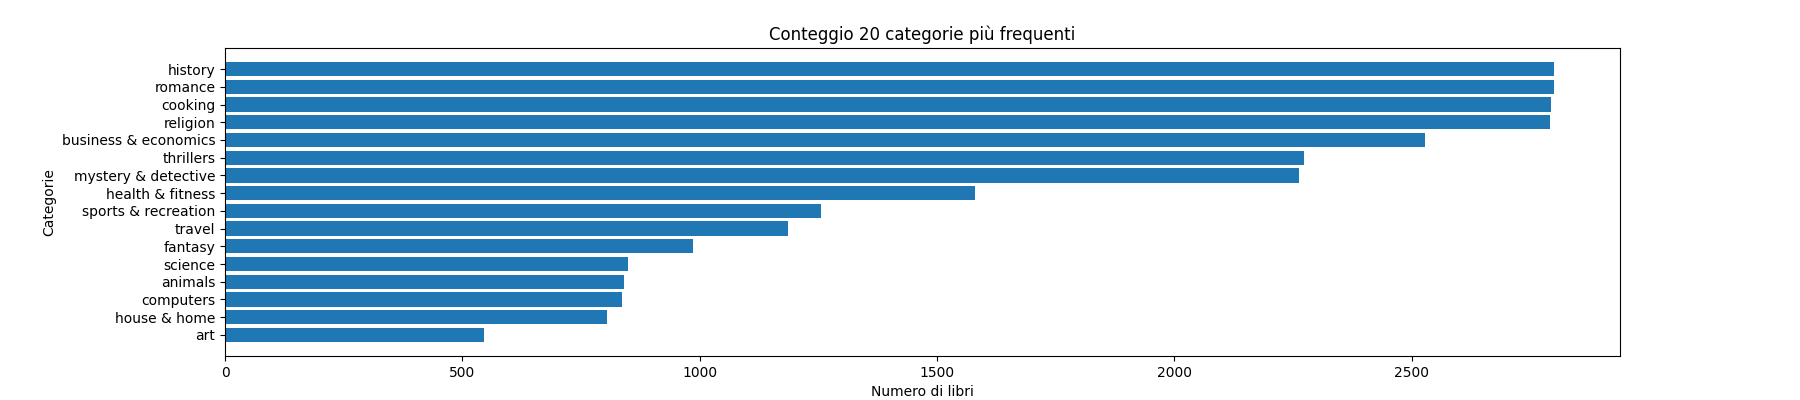
\includegraphics[width=0.96\textwidth]{dati_postprocessati.png}


    \begin{wrapfigure}{r}{0.50\textwidth}
    \begin{justify}
    Possiamo concludere che sono state effettuate le seguenti modifiche del sataset in questione, con la rimozione del seguente numero di righe:
    \end{justify}
    \includegraphics[width=0.70\textwidth, right]{bilanciamento.png}
    \caption{Didascalia dell'immagine}
    \label{fig:immagine_esempio}
    \end{wrapfigure}
    \end{enumerate}

    \begin{enumerate}
    \subsection{Visualizzazione Word Cloud}
    \end{enumerate}

    \begin{enumerate}
    \subsection{Formattazione dei dati}
    \end{enumerate}


\section{Classificazione}
    \begin{enumerate}
    \subsection{Support Vector Classification}
    \end{enumerate}
   
    \begin{enumerate}
    \subsection{Mulinomial Classification}
    \end{enumerate}
    
    \begin{enumerate}
    \subsection{Logistic Classification}
    \end{enumerate}

    \begin{enumerate}
    \subsection{SGD Classification}
    \end{enumerate}
    
    \begin{enumerate}
    \subsection{Valutazione della Classificazione}
    \end{enumerate}


\section{Clustering}
    \begin{enumerate}
    \subsection{Algoritmo K-Means}
    \end{enumerate}

    \begin{enumerate}
    \subsection{Algoritmo MiniBatchKMean}
    \end{enumerate}

    \begin{enumerate}
    \subsection{Algoritmo SpectralClustering}
    \end{enumerate}

    \begin{enumerate}
    \subsection{Valutazione del Clustering: Silhouette score}
    \end{enumerate}

\section{Conclusioni}

    
\end{document}


